\documentclass[letterpaper, 8pt]{extarticle}
\usepackage{amssymb,amsmath,amsthm,amsfonts}
\usepackage{multicol,multirow}
\usepackage{calc}
\usepackage{ifthen}
\usepackage[landscape]{geometry}
\usepackage[colorlinks=true,citecolor=blue,linkcolor=blue]{hyperref}
\usepackage{booktabs}
\usepackage{ulem}
\usepackage{enumitem}
\usepackage{tabulary}
\usepackage{graphicx}
\usepackage{siunitx}
\usepackage{tikz}
\usepackage{derivative}
\usepackage{svg}
\usepackage{listings}
\usepackage{setspace} 
\usepackage{listings}
\usepackage{xcolor}

\setstretch{0.1}
\lstset{
commentstyle=\color{blue},
morecomment=[l]{$},
}

\ifthenelse{\lengthtest { \paperwidth = 11in}}
    { \geometry{top=.25in,left=.25in,right=.25in,bottom=.35in} }
	{\ifthenelse{ \lengthtest{ \paperwidth = 297mm}}
		{\geometry{top=1cm,left=1cm,right=1cm,bottom=1cm} }
		{\geometry{top=1cm,left=1cm,right=1cm,bottom=1cm} }
	}

\newenvironment{Figure}
  {\par\medskip\noindent\minipage}
  {\endminipage\par\medskip}

\pagestyle{empty}
\makeatletter
\renewcommand{\section}{\@startsection{section}{1}{0mm}%
                                {-1ex plus -.5ex minus -.2ex}%
                                {0.5ex plus .2ex}%x
                                {\normalfont\normalsize\bfseries}}
\renewcommand{\subsection}{\@startsection{subsection}{2}{0mm}%
                                {-1explus -.5ex minus -.2ex}%
                                {0.5ex plus .2ex}%
                                {\normalfont\small\bfseries}}
\renewcommand{\subsubsection}{\@startsection{subsubsection}{3}{0mm}%
                                {-1ex plus -.5ex minus -.2ex}%
                                {1ex plus .2ex}%
                                {\normalfont\tiny\bfseries}}
\makeatother
\setcounter{secnumdepth}{0}
\setlength{\parindent}{0pt}
\setlength{\parskip}{0pt plus 0.5ex}
% -----------------------------------------------------------------------
% \tymin=37pt
% \tymax=\maxdimen

% Custom siunitx defs
\DeclareSIUnit\noop{\relax}

\NewDocumentCommand\prefixvalue{m}{%
\qty[prefix-mode=extract-exponent,print-unity-mantissa=false]{1}{#1\noop}
}

% Shorthand definitions
\newcommand{\To}{\Rightarrow}

% condense itemize & enumerate
\let\olditemize=\itemize \let\endolditemize=\enditemize \renewenvironment{itemize}{\olditemize \itemsep0em}{\endolditemize}
\let\oldenumerate=\enumerate \let\endoldenumerate=\endenumerate \renewenvironment{enumerate}{\oldenumerate \itemsep0em}{\endoldenumerate}
\setlist[itemize]{noitemsep, topsep=0pt, leftmargin=*}
\setlist[enumerate]{noitemsep, topsep=0pt, leftmargin=*}

\title{2LC3}

\begin{document}

\raggedright
\tiny

\lstset{
tabsize = 1, %% set tab space width
showstringspaces = false, %% prevent space marking in strings, string is defined as the text that is generally printed directly to the console
basicstyle = \tiny \ttfamily , %% set listing font and size
breaklines = true, %% enable line breaking
numberstyle = \tiny,
postbreak = \mbox{\textcolor{red}{$\hookrightarrow$}\space}
}

% \begin{center}
%   {\textbf{2ME3 - OSCS}} \\
% \end{center}
\setlength{\premulticols}{1pt}
\setlength{\postmulticols}{1pt}
\setlength{\multicolsep}{1pt}
\setlength{\columnsep}{2pt}
\begin{multicols*}{5}

%  \tikz[remember picture,overlay] \node[opacity=0.1,inner sep=0pt] at (current page.center){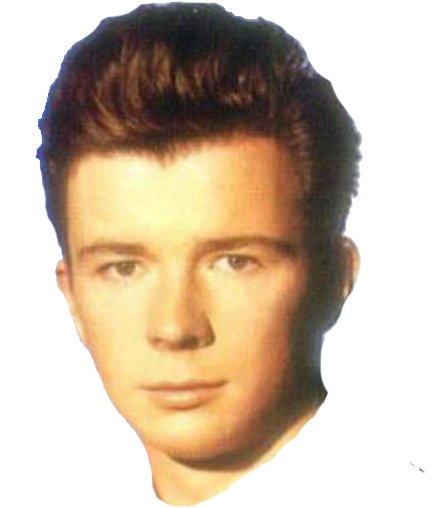
\includegraphics[height=0.8\paperheight]{makima.png}};

  \section{Programming Paradigms}
  \textbf{Procedural:} C, Assembly
  \textbf{Object-Oriented:} C\#, C++, Python, Java, Scala
  \textbf{Functional:} Haskell, Elm, Scala
  \textbf{Logical:} Prolog

  \section{CS vs SE}
  \textbf{CS:} More theory focused, Algorithms

  \textbf{SE:} Practical / Implementation, Design,
  Regulated by CEAB, not taken too seriously by PEO

  \textbf{PEO:} Professional Engineers of Ontario, Licensing and accreditation for Engineering \\
  4 years of practical experience (3 with an accredited degree), law / ethics exam, yearly fees \\
  Regulation, enforcement, discipline \\
  Has legal authority to fine companies misusing the term engineer \\
  Iron Ring just means you graduated, pretty useless, get it at the Kipling ceremony

  \textbf{CEAB:} Canadian Engineering Accreditation Board,
  determines if an engineering program gets approved.

  \section{SDLC}
  \begin{itemize}
    \item Requirement Analysis
          \begin{itemize}
            \item Getting input from stakeholders (customers, salespeople, industry experts, programmers.)
            \item What the software does
            \item Software Requirements Specification (SRS)
                  \begin{itemize}
                    \item Document describing what the software is, what it does, etc.
                  \end{itemize}
            \item Functional Requirements
                  \begin{itemize}
                    \item What the software actually does
                    \item Must be:
                          \begin{itemize}
                            \item Atomic: Each requirement should cover exactly one function of the software
                            \item Precise: Requirements should not be ambiguous
                            \item Verifiable: Must be testable to determine whether the requirement is actually met
                          \end{itemize}
                    \item Things you can \textbf{prove} using logic / discrete math
                    \item ``The software shall...''
                  \end{itemize}
            \item Non-functional Requirements
                  \begin{itemize}
                    \item Usability, performance, security
                  \end{itemize}
          \end{itemize}
    \item Specification and Design
          \begin{itemize}
            \item Determining how the software will meet requirements specified in SRS document.
            \item Modules, classes \& objects, packages
            \item Libraries \& APIs
            \item Class Diagrams
            \item What the code does, what should functions output given specific inputs
          \end{itemize}
    \item Coding
          \begin{itemize}
            \item How specification is implemented
          \end{itemize}
    \item Deployment and Maintenance
  \end{itemize}
  \subsection{Contract between client and developers}
  \textbf{Scope:} Important for clients, allows for specifying what should be included.
  \textbf{Out of scope:} Important for devs,
  allows specifying what the program will not be responsible for,
  preventing feature creep.

  \subsection{Methodologies}
  \textbf{Waterfall:} Finish one phase completely, then start the next.
  Each phase has mini-plan, and waterfalls into next.
  Drawback is that missing details in one phase
  end up causing issues in future phases.
  \begin{center}
      \includegraphics[width=0.8\linewidth]{waterfall.png}
  \end{center}

  \textbf{Agile:} Separate product into cycles
  and deliver working product quickly.
  Essentially small loops of waterfall,
  each only concerned about a small part of each step
  (eg requirements can be loose at the beginning, sprints may not produce working code).
  Constant feedback allows for issues to be spotted before they become massive problems.
  Lots of customer interaction can lead the project astray.
  \begin{center}
      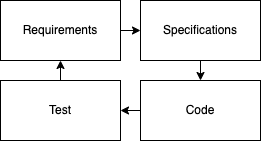
\includegraphics[width=0.6\linewidth]{agile.png}
  \end{center}

  \textbf{Spiral:} Similar to agile, but a prototype is made each sprint cycle.

  \section{Good Software}
  Efficient, timely, performant.
  \textbf{Maintainable:} Salable, Extendable, Reusable, Readable
  High Usability.
  \textbf{Reliable:} The ability of a system or component to perform
  required functions under static conditions for a specific period
  \textbf{Correctness:} Meets (specified) requirements.
  Correctness is achieved if it behaves exactly as intended
  for all of its use-cases. (eg passes tests)
  \textbf{Robust:} Meets unspecified requirements.
  The ability of a system to cope with errors during execution,
  and cope with erroneous input (eg the program should fail gracefully)
  \textbf{Distribution of cost in development}
  40\% of cost on initial development. 60\% on maintenance.
  Of that, 20\% is on making sure things are correct,
  20\% is adaptive (correcting things the client wants to be fixed),
  20\% is improvement.

  \section{Object-Oriented Programming}
  \subsection{Encapsulation}
  Safeguarding the content of a class from direct outside access.
  Make certain fields private, access them through public getters and setters.
  Separation of concerns.
  \textbf{Modularity:} Programs should be made up of independent, interchangeable parts
  Information Hiding
  Single responsibility Principle
  \textbf{Open-close principle:} objects should be open for extension,
  but closed for modification.

  \subsection{Relationships between Classes}
  \subsubsection{Inheritance}
  Is-a relationship. Good for reusability, code does not need to be rewritten.
  \subsubsection{Aggregation}
  Has-a relationship: A has-a B, then A has an instance of B.
  Must be mandatory upon creation, otherwise it is simply association / dependence
  \subsubsection{Composition}
  Part-of relationship: A part-of B, A can't exist without B, and vice-versa.
  A subset of aggregation.
  \subsubsection{Dependence / Association}
  Uses-a relationship: A uses-a B, then A creates an object of B inside a method.
  Association is generally between unrelated classes. % check this, not too certain

  \subsection{Abstraction}
  Hides complexity from users, showing only relevant info.
  Implementation hidden using abstract (partially abstract) classes,
  or interfaces (fully abstract).

  \subsection{Polymorphism}
  Performing a certain action in different ways (eg animals can make different noises).
  \textbf{Method overloading:} various methods with the same name but different parameters.
  \textbf{Method overriding:} child class overrides a method of its parent.

  \section{UML Diagrams}
  \begin{center}
    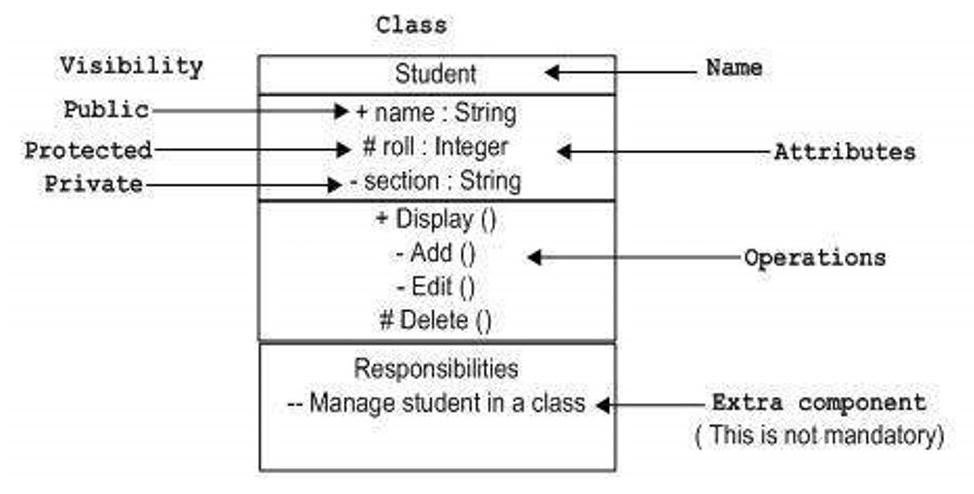
\includegraphics[width=.9\linewidth]{uml-class.png}
    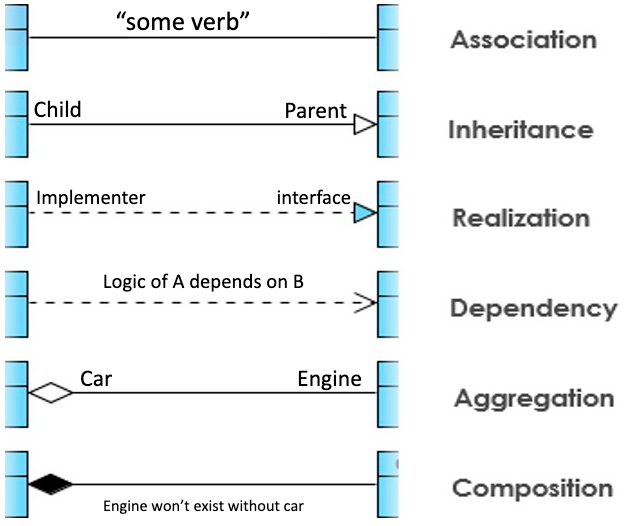
\includegraphics[width=.7\linewidth]{uml-arrows.png}
  \end{center}

  \section{Java}
  \subsection{Abstract Class}
  Can have abstract and non-abstract method.
  Can have non-final variables
  Can have final, non-final, static, and non-static variables.
  Can provide implementation of abstract class.
  Uses ``extends''
  Can only extend one other class, but can implement multiple interfaces.
  Does not support multiple inheritance.
  Can have private members.
  \subsection{Interface}
  Can only have abstract methods.
  Variables are final by default.
  Can only have static and final variables.
  Can't provide implementation of abstract class.
  Can extend one or more Java interfaces.
  Supports multiple inheritance.
  Members are public by default.

  \section{Multiple Inheritance}
  When a class inherits from more than one class.
  Constructors are called in the order they are inherited.

  \section{SOLID}
  \textbf{Single responsibility principle:}
  Each class should have one and only one responsibility.

  \textbf{Open/Closed Principle:}
  Classes should be open for extension but closed for modification

  \textbf{Liskov's Substitution Principle:}
  Parent classes should be easily substituted with child classes without
  the application malfunctioning.
  \textbf{Interface Segregation Principle:}
  Many client-specific interfaces are better than one general interface.
  \textbf{Dependency Inversion Principle:}
  Classes should depend on abstraction, but not on concretion.
  Aka, have an interface which allows for communication with concrete classes.
  If class A changes, class B should not be affected.

  \section{Design Principles}
  \subsection{Information Hiding}
  AKA Single Responsibility Principle
  AKA Encapsulation

  Changes to a class should have \textbf{minimal} impact on other code:
  The API for a class should be completely independent of the implementation.

  \subsection{Open-Closed}
  Entities should be open for extension, but closed for modification.

  In other words, the original functionality should remain static,
  while allowing new functionality to be added on,
  without the original source needing to be modified.

  \subsection{Design for Interfaces}
  AKA Dependency Inversion
  Don't depend on concrete classes, use interfaces instead.

  \section{Creational Patterns}
  \subsection{Factory}
  Provides an interface for creating objects in a superclass,
  allows subclasses to alter type of objects that will be created.
  Eg: Pizza, Shapes, Ingot
  \begin{enumerate}
    \item Have an interface A
          \begin{lstlisting}[language=Java, breaklines=true]
public interface Factory {
  public Enemy spawn();
}
        \end{lstlisting}
    \item Have factory ``products'' implement A
          \begin{lstlisting}[language=Java, breaklines=true]
public abstract class Enemy {
  protected int health;
  protected int strength;
  public abstract void takeDamage(int damage);
  public abstract void attack();
}
        \end{lstlisting}
    \item Have the factory function return an object of type A
          \begin{lstlisting}[language=Java, breaklines=true]
public class AverageSpawner implements Factory{
  @Override
  public Enemy spawn() {
    Random r = new Random();
    double k;
    k = r.nextDouble();
    if(k < 0.65) {return new Minion();}
    else if(k < 0.9) {return new Elite();}
    else {return new Boss();}
  }
}
        \end{lstlisting}
    \item Let clients get ``products'' through the factory function
  \end{enumerate}

  \begin{center}
    % \includegraphics[width=0.9\linewidth]{factory.png}
    \includegraphics[width=0.9\linewidth]{factory-example.png}
  \end{center}

  \textbf{Advantages:}
  Can switch out factories at runtime to change what's being produced.
  Object instantiation is encapsulated.
  Single Responsibility Principle - can move product creation into a separate area,
  making code easier to support.
  Open Closed Principle - can introduce new types of products without
  affecting existing code.

  \textbf{Disadvantages:}
  Code can become complex due to subclasses.

  \subsection{Singleton}
  Creational patter that ensure that class has only one instance, while providing a global access point to instance.
  \begin{center}
      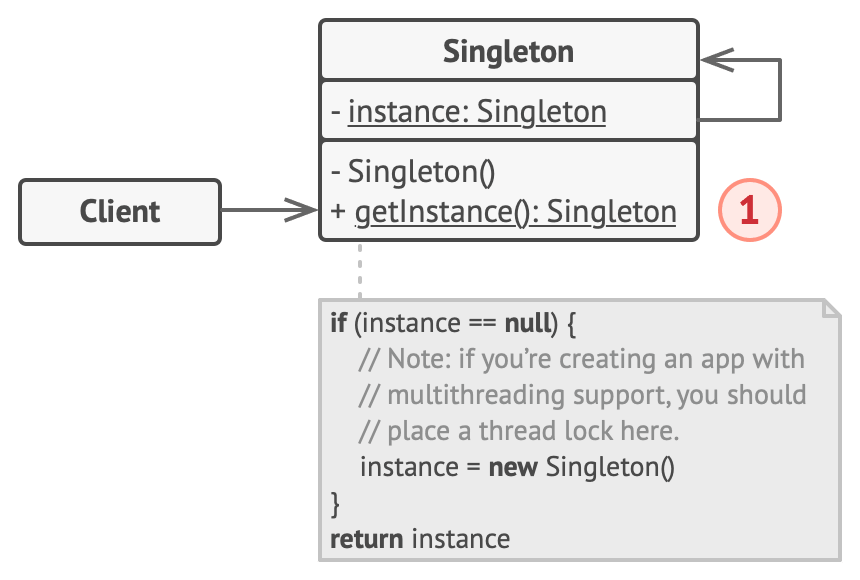
\includegraphics[width=.7\linewidth]{singleton.png}
  \end{center}
  \begin{lstlisting}[language=Java, breaklines=true]
public class TheOne {
  private static TheOne instance;
  public static TheOne getInstance() {
    if(instance == null) {
      instance = new TheOne();
    }
    return instance;
  }
  private TheOne() {}
}
  \end{lstlisting}
  \textbf{Advantages:}
  Guaranteed that class has only one instance.
  Global access point to single instance.
  Initialized only when needed (lazy).

  \textbf{Disadvantages:}
  Violates SRP: solves two problems at once (ensure class has only one instance, and providing global access point to instance).
  Can make for bad design, eg when components know too much about each other.
  Can be difficult to unit test client code, as frameworks rely on inheritance when mocking.
  % TODO: add singleton
  

  \section{Structural Patterns}
  \subsection{Decorator}
  Lets you attach new behaviors to objects by putting them in special wrappers
  that contain the behaviors. Eg: Starbucks, Burgers

  \begin{enumerate}
    \item Create interface A
          \begin{lstlisting}[language=Java, breaklines=true]
public interface Burrito {
  public double getCost();
  public String getString();
}
        \end{lstlisting}
    \item Create base class B that implements A
          \begin{lstlisting}[language=Java, breaklines=true]
public class ChickenBurrito implements Burrito{
  public ChickenBurrito() {}
  public String getString() {
    return "Chicken" + "$12.00";
  }
  public double getCost() {
    return 12.00;
  }
}
        \end{lstlisting}
    \item Create decorator class C that implements A,
          that holds an instance of B,
          which is received through constructor
          \begin{lstlisting}[language=Java, breaklines=true]
public abstract class BurritoDecorator implements Burrito {
  protected Burrito burrito;
  public BurritoDecorator(Burrito burrito) {
    this.burrito = burrito;
  }
  @Override
  public abstract double getCost();
  @Override
  public abstract String getString();
}
        \end{lstlisting}
    \item Create decorators by extending C and using super
          \begin{lstlisting}[language=Java, breaklines=true]
public class Guac extends BurritoDecorator {
  public Guac(Burrito burrito) {
    super(burrito);
  }
  @Override
  public double getCost() {
    return 1.50 + burrito.getCost();
  }
  @Override
  public String getString() {
    return burrito.getString() + "\n--Guac + "$1.50";
  }
}\end{lstlisting}
  \end{enumerate}

  \begin{center}
    % \includegraphics[width=0.8\linewidth]{decorator.png}
    \includegraphics[width=0.8\linewidth]{decorator-example.png}
  \end{center}

  Decorators are both the original component, and also use the original component.

  \textbf{Advantages:}
  Extensibility of code, new decor can just extend decorator interface.
  Greater flexibility, able to add or remove decorators at runtime.
  Simplifies coding, don't have to put all the functionality into the object.
  Single Responsibility Principle, larger classes can be broken down into several smaller ones.

  \textbf{Disadvantages:}
  Code can be harder to maintain, decreases as number of decorator classes grows.
  Hard to remove wrappers.
  Hard to implement decorators in a way that doesn't depend on ordering. E.g. Bird/Duck, Car/Boat

  \subsection{Adapter}
  % TODO: add adapter UML Diagram
  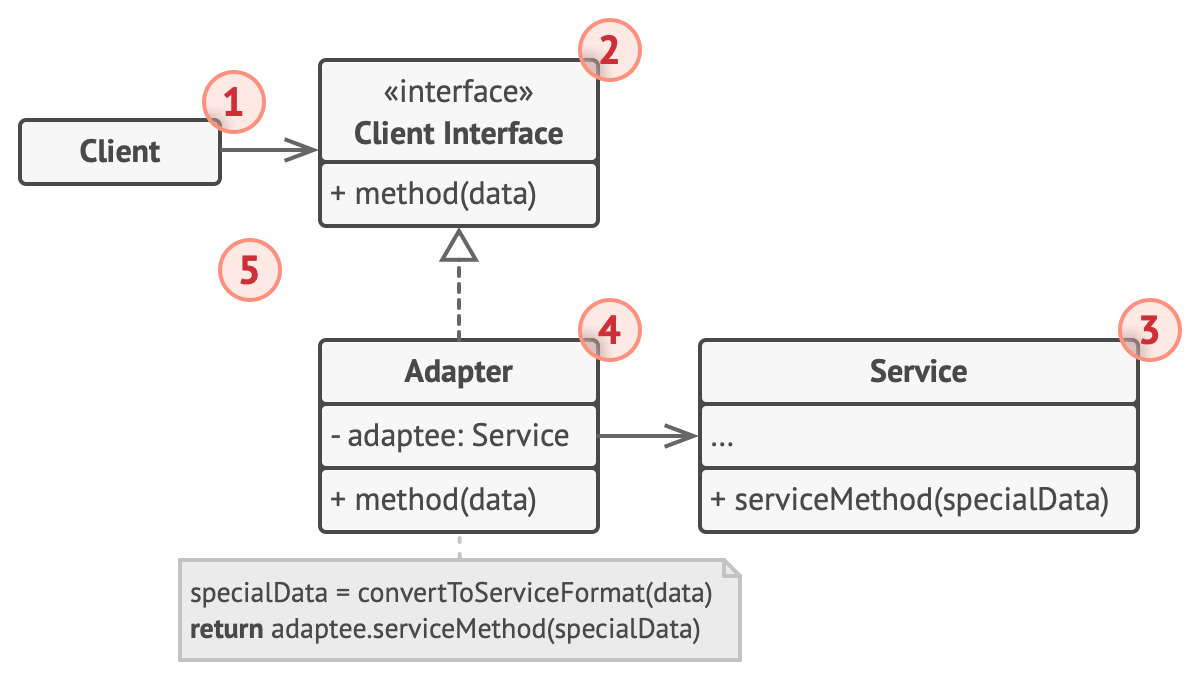
\includegraphics[width=\linewidth]{adapter.png}
  \begin{lstlisting}[language=Java, breaklines=true]
public class Hospital {
  private Patient[] currentPatients = new Patient[100];
  private MedOffice requester;
  public void bookPatient(int index, Date date) {
    requester.registerPatient(currentPatients[index]);
  } 
}
public interface MedOffice {
  public void registerPatient(Patient patient);
}
public class MedOfficeAdapter implements MedOffice{
  private ActualMedOffice office = new ActualMedOffice();
  @Override
  public void registerPatient(Patient patient) {
    office.registerPatient(patient.getName(), patient.getId());
  }
}
public class ActualMedOffice {
  public void registerPatient(String name, int id) {} 
}
  \end{lstlisting}
  Works as a bridge between two incompatible interfaces. A single class converts the interface of one object so that another object can understand it.
  \textbf{Advantages} Single Responsibility Principle: You can separate the interface or data conversion code from the primary business logic of the program. Open/Closed Principle: You can introduce new types of adapters into the program without breaking the existing client code, as long as they work with the adapters through the client interface.
  \textbf{Disadvantages} Overall complexity of code increases because you need to introduce a set of new interfaces and classes. Sometimes it’s simpler just to change the service class so that it matches the rest of your code.

  \subsection{Proxy}
  % TODO: add proxy
  Lets you substitute or placeholder for another object. \textbf{Controls access} to original object,
  allowing for actions before / after request gets through.Proxy is used as a security to emulate the service so that the client cant access the service directly (think of an ATM, we dont want people to have access to the actual money numbers, just a representation of them).
  Eg: Database proxy, Discord Example
  \begin{center}
      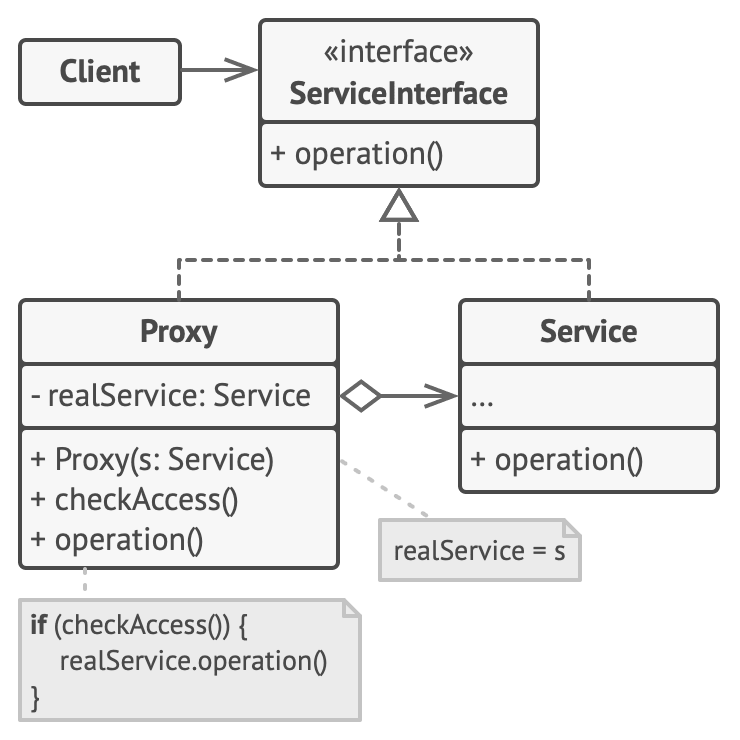
\includegraphics[width=.6\linewidth]{proxy.png}
  \end{center}
  \begin{lstlisting}[language=Java, breaklines=true]
RealDiscordServer adm = new RealDiscordServer("2ME3");
ProxyDiscordServer usr = new ProxyDiscordServer(adm);
User a = new User("j", usr);
User admin = new User("a", adm);
public class User {
  String username;
  DiscordServer ds;
  public User(String u, DiscordServer ds) {
    username = u;
    this.ds = ds;
  }
  public void sentAMessage(String s) {
    ds.sendMessage(s);
  }
  public void getAMessage() {
    ds.recieveMessage();
  }
  public void banPlayer(String s) {
    ds.banUser(s);
  }
}
public interface DiscordServer {
  public void banUser(String s);
}
public class ProxyDiscordServer implements DiscordServer {
  DiscordServer ds;
  public ProxyDiscordServer(DiscordServer ds) {
    this.ds = ds;
  }
  @Override
  public void banUser(String s) {
    if (s.length() > 10) {
      ds.banUser(s);
    }
  }
}
public class RealDiscordServer implements DiscordServer {
  String name;
  public RealDiscordServer(String name) {
    this.name = name;
  }
  @Override
  public void banUser(String s) {
    System.out.println("Banned: " + s);
  }
}
  \end{lstlisting}
  \textbf{Advantages}
  Can control service object without clients knowing
  Can manage lifecycle of service object isn't ready or isn't available.
  Open/Closed Principle You can introduce new proxies without changing service or clients.
  \textbf{Disadvantages}
  Code can become more complicated since new classes are introduced.
  Response from service may be delayed.

  \section{Behavioral Patterns}
  \subsection{Strategy}
  Define a family of algorithms, put them each in separate classes,
  and make their objects interchangeable. E,g. Weapon (Fist, Sword)
  \begin{enumerate}
    \item Create a strategy interface
          \begin{lstlisting}[language=Java, breaklines=true]
public interface Sorter {
  public void sort(ArrayList<Double> data);
}
        \end{lstlisting}
    \item Create concrete strategies that implement the interface
          \begin{lstlisting}[language=Java, breaklines=true]
public class DefaultSorter implements Sorter{
  @Override
  public void 
    sort(ArrayList<Double> data) {
    Collections.sort(data);
  }
}
        \end{lstlisting}
    \item Create a context to store the strategy
          \begin{lstlisting}[language=Java, breaklines=true]
public class SensorData {
  private ArrayList<Double> data = new ArrayList<Double>();
  private Sorter sort;
  public SensorData() {
    sort = new DefaultSorter();
  }
  public void addValue(double value) {
    data.add(value);
  }
  public void setSort(Sorter sort) {
    this.sort = sort;
  }
  public void sort() {
    sort.sort(data);
  }
}

        \end{lstlisting}
  \end{enumerate}
  \begin{center}
    % \includegraphics[height=3.5cm]{strategy.png}
    \includegraphics[width=0.9\linewidth]{strategy-example.png}
  \end{center}

  \textbf{Advantages:}
  Open-Closed Principle - Introducing new strategies without changing the encapsulation code,
  hiding of algorithm from application.
  Algorithms used by object can be changed at runtime.
  More maintainable, usable, extensible.

  \textbf{Disadvantages:}
  Overly complex if there are only a few algorithms needed.
  Must be aware of the difference between algorithms to pick the right one.

  \subsection{Observer}
  % TODO: add java code
  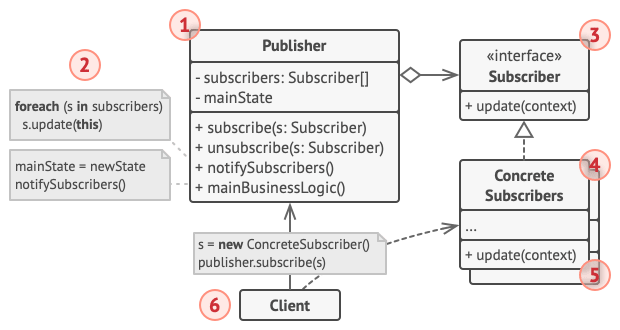
\includegraphics[width=\linewidth]{observer.png}
  Pull $\rightarrow$ --
  Push $\rightarrow$ !!
  \begin{lstlisting}[language=Java, breaklines=true]
public interface Subject {
  public void add(Observer o);
  public void remove(Observer o);
  public void update(!String s!);
}
public class Course implements Subject {
  String courseName;
  String courseAnnouncement;
  ArrayList<Observer> students;
  public Course(String courseName) {
    this.courseName = courseName;
    courseAnnouncement = "";
    students = new ArrayList<Observer>();
  }
  @Override
  public void add(Observer o) { students.add(o); }
  @Override
  public void remove(Observer o) { students.remove(o); }
  @Override
  public void update(!String s!) { for (Observer o : students) { o.update(!String s!); } } }
  public interface Observer { public void update(); }
  
  public class Student implements Observer {
    String name;
    -Course course;-
    String courseAnnouncement;
    public Student(String name, -Course course-) {
      this.name = name;
      -this.course = course;-
      -enroll();-
    }
  @Override
  public void update(!String s!) {
    -courseAnnouncement = course.courseAnnouncement;-
    !courseAnnouncement = s;!
  }
  -public void enroll() {
    System.out.println(name + " enrolled in " + course.getCourseName());
    course.add(this);-
  }
  -public void drop() {
    System.out.println(name + " dropped " + course.getCourseName());
    course.remove(this);-
  }
}
  \end{lstlisting}
  Publisher calls update() on subscribers when needed. Subscribers can be added or removed at runtime. Push: when update() is called, the observers directly get the data from the function. Pull: when update is called, subject.getState() is used to get the data instead.
  \textbf{Advantages:} Open-Closed Principle, can add new subscribers without changing the publisher.
  Can establish Relationships between objects at runtime.

  \textbf{Disadvantages:} Subscribers are notified in random order.
  \textbf{Push:} Observer is notified that a change has occurred and must find out itself what changes have occurred. Used when all the observers are interested in common state changes. Not used for large amounts of data. No need for getState().(Advantage)Suppliers generate events and actively pass them to an event channel. 
  \textbf{Pull:} The subject sends observers detailed information about the change that has occurred(in the simplest case, the entire new state itself). No parameter for the state in update() but need getstate() for subject construct class.This can lead to further requests from the observer to the subject. More than one call is required $\rightarrow$ change notification from the subject to all its observers $\rightarrow$ interested observer must call at least one method to pull data. (Advantage)simpler to write, and work when the client application is hosted behind a firewall (traffic is outbound). 

  \subsection{Command}
  % GRRRRRRRRRRR WOOF WOOF BARK BARK ARF BARK GRRRR WOOF SNARL HSSSS GRRRR WOOF WOOF BARK ARF GRRRR HSSSS WOOF WOOF BARK ARF GRRRRR HSSSSS BARK ARF GRRRR WOOF WOOF BARK GRRR SNARL ARF WOOF BARK ARF SNARL HSSSSSS he jus like me fr
%  \tikz[remember picture,overlay] \node[opacity=0.1,inner sep=0pt] at (current page.center){
\includegraphics[height=0.8\paperheight]{346653161077211.png}};
  % TODO: add command
  Turns a request into a stand-alone object containing all information about request.
  Allows requests to be passed as method arguments, delay or queue a request's execution, and undo operations.
  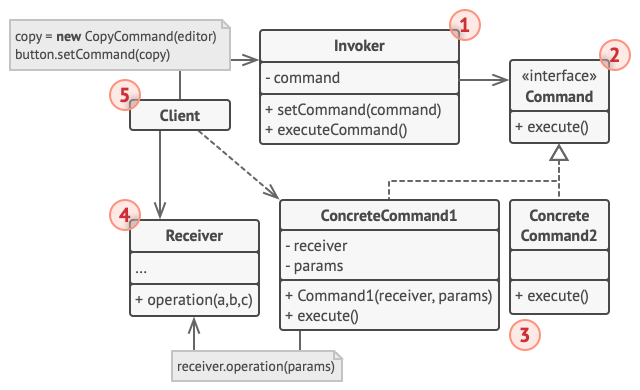
\includegraphics[width=\linewidth]{command.png}
    \begin{lstlisting}[language=Java, breaklines=true]
public class Remote {
  Stack<Command> commands;
  public Remote() { commands = new Stack<Command>(); }
  public void execute(Command c) { commands.add(c); c.execute(); } 
}
public interface Command { public void execute(); }
public class LightON implements Command {
  Light l;
  public LightON(Light l) { this.l = l; }
  @Override
  public void execute() { l.turnOn(); }
}
public class Light {
  boolean isOn;
  String name;
  public Light(String name) {
    isOn = false;
    this.name = name;
  }
  public void turnOn() { isOn = true; }
  public void turnOff() { isOn = false; }
}
    \end{lstlisting}
  \textbf{Pros:} \textbf{Single Responsibility Principle:} decoupling classes that invoke ops from classes that perform ops
  \textbf{Open/Closed Principle:} Introducing new commands into app without breaking existing client code
  Implement undo/redo.
  Implement deferred execution of operations.
  Assemble set of simple commands into a complex one.
  \textbf{Cons:} Code becomes more complicated as new layer exists between senders and receivers

  \section{Formal Specification}
  Form: $(\forall x : \mathbb{N} \mid R : P)$,
  where $\forall$ is a quantifier, $x$ is a variable, $\mathbb{N}$ is the type of variable,
  $R$ is the range over which the predicate is to be executed, and $P$ is the predicate.

  \subsection{Formal Spec examples}
  \begin{itemize}
  \setlength\itemsep{0.9em}
    \item Checks if a list L contains x
    $(\exists i \mid 0 \leq i < |L| : x = L [I])$
    \item Counts the amount of times x appears in list L
    $(\sum i \mid 0 \leq i < |L| \land L[i] = x: 1)$
    \item Checks if a list is a sorted copy of another
    $(\forall i: \mathbb{N} \mid (0 \leq i < |L_1| - 1): L_1[i] \leq L_1[i + 1]) \land (\forall i : \mathbb{N}|: count(L, i) = count(L_1, i))$
    \item Checks if there's a duplicate name in a set of users
    $(\forall x,y: User \mid (x \in myUserSet \land y \in myUserSet) \land (x \neq y) : (x.username \neq y.username))$
    \item Checks if two circles overlap
    $(getPoints(this) \cup getPoints(c)) \neq 0$
    \item All people have less than 10 children
    $(\forall p_1 : Person \mid p_1 \in people : (\sum p_2 : Person \mid p_2 \in people: \textit{Children}(p_1, p_2) \leq 10)$
    \item returns set of friendships associated with friend (s)
    $ getfriends(s) = {friend:String:X(s,friend)\in Friendships}$
    \item Gives set of friends of friends
    $(\cup (friend : String \mid friend \in getFriends(getFriends(s)) : friend)-{s}-getfriends(s)$
    \item
    $(\cup (friend : String \mid friend \in getFriends(getFriends(s)) : friend)-{s}-getfriends(s)$
    \item Gives set of friends of friends
    $(\cup (friend : String \mid friend \in getFriends(getFriends(s)) : friend)-{s}-getfriends(s)$
    \end{itemize}
  \subsection{Valid Group Exercise Example}
  \begin{itemize}
  \setlength\itemsep{0.9em}
  \item Types
    Student = Tuple(id:String,gender:String, discipline:string, section:$Z$), Team = Student{}, Classlist:Student{}, Teams:Teams{}
    \item Everyone in the teams, is enrolled in the course
    $(\forall t:Team \mid t \in Teams: 4 \leq |t| \leq 6)$
    \item Each student enrolled in the course is in a team
    $(\forall s:Student \mid s \in Classlist: (\exists t: Team \mid t \in Teams: s \in t))$
    \item No student appears in two different teams exactly one team
    $(\forall s:Student \mid s \in Classlist: (\forall t_1,t_2: Team \mid t_1,t_2 \in Teams: s \in t \land s \in t_2 \rightarrow t_1 = t_2))$
    \item No student appears in two different teams exactly one team
    $(\forall s:Student \mid s \in Classlist: (\forall t_1,t_2: Team \mid t_1,t_2 \in Teams: s \in t \land s \in t_2 \rightarrow t_1 = t_2))$
    \item All teams have 4 to 6 students
    $(\forall t:Team \mid t \in Teams: 4 \leq |t| \leq 6)$
    
    \end{itemize}
  
  

  \subsection{MIS}
  \subsubsection{Uses}
  \begin{itemize}
      \item Imported constants, data types, and access programs
  \end{itemize}
  \subsubsection{Syntax}
  \begin{itemize}
      \item Exported constants
      \item Exported types
      \item Exported access routine (routine name, input and output parameter types, exceptions in a table)
  \end{itemize}
  \subsubsection{Semantics}
  \begin{itemize}
    \item State variables (global variables)
    \item State invariants (predicates using state variables where after every access routine call, should remain true)
    \item Assumptions
    \item Access routine semantics
    \begin{itemize}
        \item transition = changing state variables (eg transition: this.start, this.end := start, end)
        \item output = output of access routine (eg output: out := this)
        \item exception = exception (eg exception: none)
    \end{itemize}
    \item Local functions, types, constants (used for specification only, not used at runtime)
    \item Other considerations (eg consider doing x to y to do z)
  \end{itemize}
  \begin{tabulary}{\linewidth}{@{}LL@{}}
  \toprule
    Program Specification (what it does) & Implementation (how it does it) \\ \midrule
    Math/logic & Code/computers \\
    Natural numbers/Integers & int \\
    Real numbers & Doubles, floats \\
    Strings & Strings \\
    Sets & Sets, collections, adapted lists etc. \\
    Sequences & Lists, arrays, array lists etc. \\
    \bottomrule
  \end{tabulary}

  \section{Testing}
  \textbf{V-Model:} Verification and Validation model. Associates each testing stage with its corresponding development stage. The next
  step only starts once the previous step is complete.
  \begin{center}
    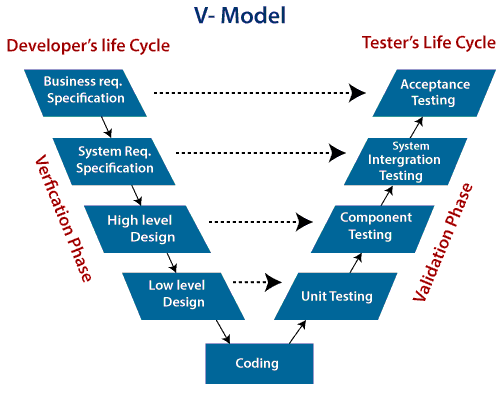
\includegraphics[width=\linewidth]{V-Model.png}
  \end{center}
  \textbf{Unit Testing:} Test individual methods / functions, with provided input expect certain output.
  \textbf{Black Box:} Test without knowledge of the code (generally check functionality, edge cases)
  \textbf{White Box:} Test with knowledge of the code
  \textbf{Code Graph:} Graph of the code, each node is a statement, each edge is a branch.
  \textbf{Statement Coverage:} Test cases cause each statement to be executed at least once.
  \textbf{Edge Coverage:} Test cases cause each edge of each decision (each branch of if statements) to be executed at least once. 1 for if and else together
  Test suite has statement coverage $\Leftrightarrow$ has edge coverage.
  There are cases where edge coverage is not enough to prove that the program works
  (eg if variables are being modified)
  \textbf{Path Coverage:} Test cases cause each path through the program to be executed at least once (each possible combination of edges). 1 for each if and else
  \textbf{Static Testing:} Test without running the program (reading code)
  \textbf{Dynamic Testing:} Test by running the program (unit testing)

  \subsection{Number of bugs}
  15 - 50 bugs per 1000 lines of code. \\
  If $N$ is the actual number of bugs, one team (markers) found $M$ bugs, another team (catchers) found $C$ bugs, and there were $S$ bugs in common,
  then the actual number of bugs ranges between $N_1 = (C - S) \frac{M}{S}$ to $N_2 = (M - S) \frac{C}{S}$.
  This assumes that $\frac{M}{S} = \frac{N}{(C-S)}$, aka the ratio of marked bugs to marked bugs caught resembles actual bugs to caught actual bugs. Might not be true though, since marked bugs are easier to catch.

  \subsection{Fault Seeding}
  Intentionally adding issues into code to try to determine how many issues are caught. See above for the formula used.
  Not necessarily accurate, as seeded issues are probably more likely to be discovered, as they are likely easier to implement. 

\end{multicols*}

\end{document}
